\documentclass{article}

\usepackage[utf8]{inputenc}
\usepackage[dvipsnames]{xcolor}
\usepackage{lmodern}
\usepackage{graphicx}
\usepackage{longtable}
\usepackage{tabularx}
\graphicspath{ {../images/} }
\usepackage{imakeidx}
\makeindex[columns=3, title=Alphabetical Index, intoc]

\usepackage{tabularx}
\usepackage{amsmath}
\usepackage{paralist}
\usepackage{enumitem}
\usepackage{hyperref} %\usepackage[hidelinks]{hyperref} %per togliere bordi rossi
\usepackage{makecell}
\usepackage{caption}
\usepackage[maxfloats=256]{morefloats}
\maxdeadcycles=1000

\usepackage[official]{eurosym}
\DeclareUnicodeCharacter{20AC}{\euro{}}

\author{Agosta, Belli, Emili, Giacchini, Luciani}

\begin{document}

\begin{center}
    \sffamily{\fontsize{50}{48} \selectfont \textcolor{red}{Nexi}\textcolor{green}{Fy}}
\end{center}

\begin{center}
    \itshape{\fontsize{20}{48} \selectfont streaming to your pocket}
\end{center}

\bigskip\bigskip\bigskip

\begin{flushleft}
    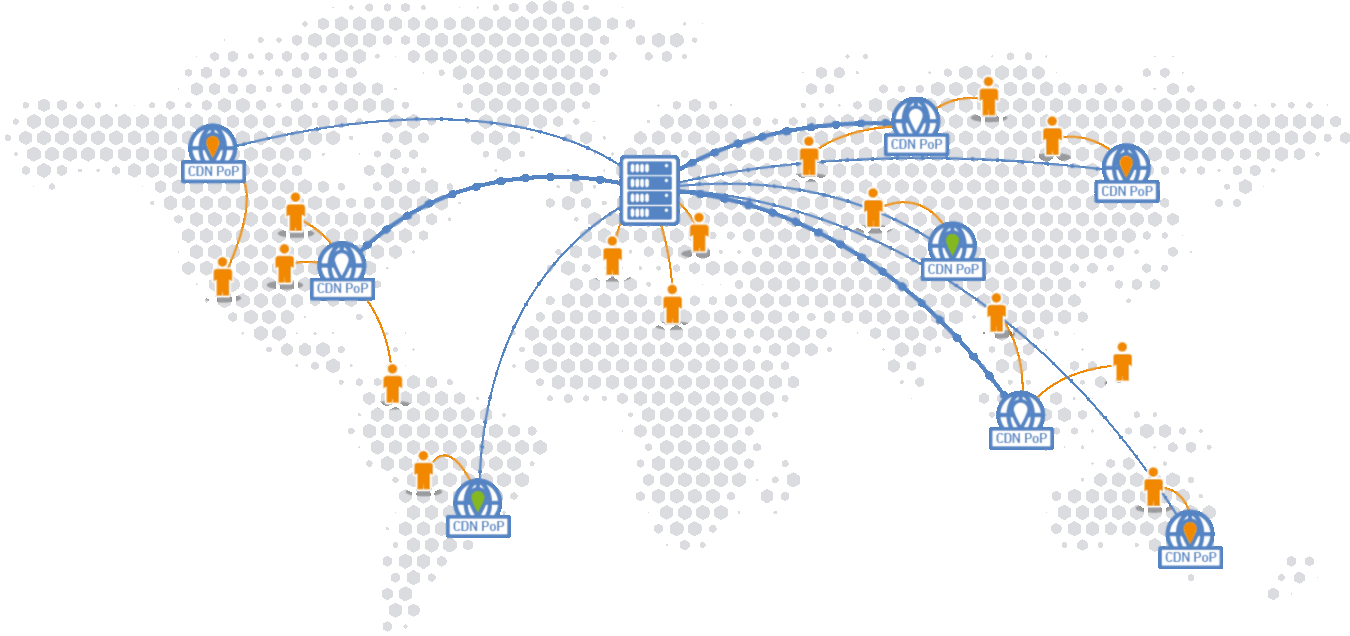
\includegraphics[scale=1]{../images/worldCDN.png}
\end{flushleft}

\bigskip\bigskip\bigskip

\begin{center}
    \itshape{\fontsize{30}{48} \selectfont Glossario}
\end{center}

\newpage
\printindex

\newpage
\section{\itshape{Glossario}}
 In questa sezione saranno esplicitati tutti i termini necessari alla comprensione del progetto.

\begin{itemize}
	%\item  \textbf{multimedia-manager}: servizio usato da partner per la gestione (caricamento/eliminazione) dei propri video e/o tracce audio. %viene citato solamente qui nel glossario
	\item \textbf{Piano di abbonamento}: pacchetto di funzionalità, acquistabile dagli utenti per un certo periodo (e rinnovabile alla fine del periodo). A volte è indicato impropriamente come "abbonamento"
	\item \textbf{API}: interfaccia offerta all'esterno di un sistema, per poter usare delle funzionalità interne al sistema
	\item \textbf{CDN}: sistema di server largamente distribuita, usata per la distribuzione di contenuti quali tracce video e audio.
	\item \textbf{ORM}: tecnica per interfacciarsi con basi di dati relazionali, astraendo dall'implementazione del dbms
	\item \textbf{Piattaforma}: componente del sistema accessibile dagli utenti.
	\item \textbf{Server}: macchina logica (composta da uno o piu macchine fisiche) su cui risiede la piattaforma in parte o nella sua totalità.
	\item \textbf{RUP}: Rational Unified Process, processo di sviluppo basato su fasi temporali, iterazioni e attività.
	\item \textbf{Risorsa Multimediale}: intendiamo un file di tipo multimediale, quindi un video, una canzone, ecc. (a volte è indicata solamente come risorsa)
	\item \textbf{Prodotto}: si intende un singolo prodotto video o audio creato da un partner (e.g: un singolo film, una singola canzone, un singolo episodio di una serie tv, ecc.)
	\item \textbf{Playlist}: lista ordinata di prodotti
	\item \textbf{Contenuto}: un singolo prodotto o una playlist
\end{itemize}
\index{Index}

\end{document}
